%!TEX root = ../main.tex
\chapter{CALICE Calorimeter concepts}

The CALICE Collaboration is developing and testing electromagnetic and hadronic calorimeters. These detector concepts are optimized toward a linear collider environment such as the International Linear Collider (ILC) \cite{Behnke:2013lya} or Compact Linear Collider (CLIC) \cite{2012arXiv1202.5940L} but collaboration with the Large Hadron Collider community for the High-Lumi upgrade (HL-LHC) is ongoing \cite{1748-0221-12-01-C01042}. The CALICE calorimeters are high granularity calorimeter optimized for the particle flow algorithm (Pandora PFA) providing a very detailed image of physics events.\\
Several prototypes for physics were build in the past and tested in testbeam campaigns at DESY, CERN and FNAL \cite{1748-0221-3-08-P08001, 1748-0221-5-05-P05004, 1707.07126v2, 1748-0221-10-10-P10039, 1748-0221-3-05-P05001}. Three physics prototypes of 1 m$^3$ were conceived using different active material and absorbers as well different readout schemes.\\
Nowadays, the CALICE Collaboration is still performing analysis on the data collected by these prototypes \cite{OskarCAN, YasmineCAN}. Also, the collaboration is looking forward in the integration into a full linear collider detector by designing several new technological calorimeter prototypes.\\
In this chapter, the electromagnetic and hadronic calorimeter concepts will be introduced, described and compared in details.

\section{Electromagnetic Calorimeters}

The CALICE Collaboration is developing two different electromagnetic calorimeters (ECAL) concepts. Physics prototypes whose goal was to prove the performance of such calorimeters for detailed measurements of EM showers, were first built. Now engineering prototypes are designed in order to improve the calorimeter design, the integration of the front-end electronics and the readout scheme. In the next subsections, the silicon-based SiECAL and the scintillator-based ScECAL calorimeters using both tungsten as absorber material will be described.

\subsection{SiECAL}

The SiECAL physics prototype consists of 30 active and absorber layers. The sensitive layer is made of high-resistivity silicon wafers 525 \si{\micro\meter} thick. These are divided in 6$\times$6 cm$^2$ sensors, segmented into a matrix of 1$\times$1 cm$^2$ PIN diodes operated in reversed bias. The total active area is 18$\times$18 cm$^2$ which resulted in 9720 channels. The depth of the calorimeter was 24 X$_0$ achieved by 10 layers of 0.4 X$_0$ (1.4 mm), followed by 10 layers of 0.8 X$_0$ (2.8 mm) and 10 more layers of 1.2 X$_0$ (4.2 mm) thick tungsten absorber plates. No front-end electronics was integrated into the layers but placed off-detector using analog lines. The performance of such calorimeter was tested in various beams at DESY and CERN. An energy resolution of $\frac{16.53\%}{\sqrt{E}}$ stochastic term and $1.07\%$ constant term was achieved \cite{ADLOFF2009372}.

\begin{figure}[htbp!]
  \centering
  \begin{subfigure}[t]{0.49\textwidth}
    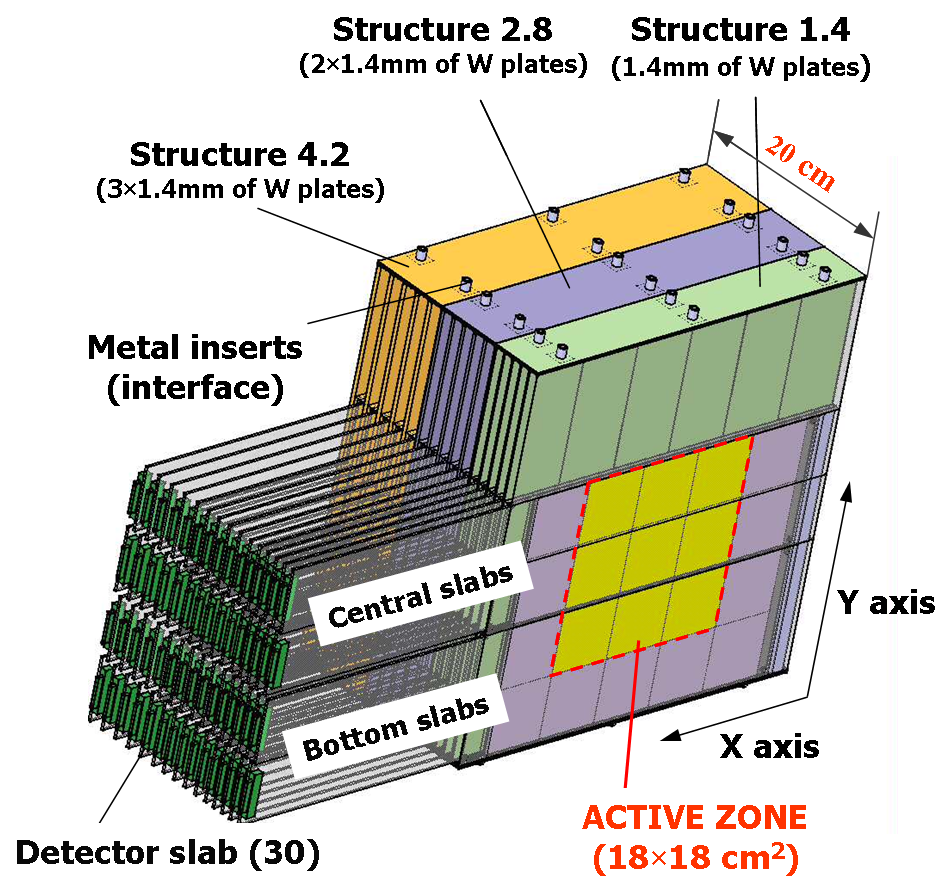
\includegraphics[width=1.\linewidth]{chap3/fig/3DProtoH.png}
    \caption{} \label{fig:SiWECALPhysics}
  \end{subfigure}
  \hfill
  \begin{subfigure}[t]{0.49\textwidth}
    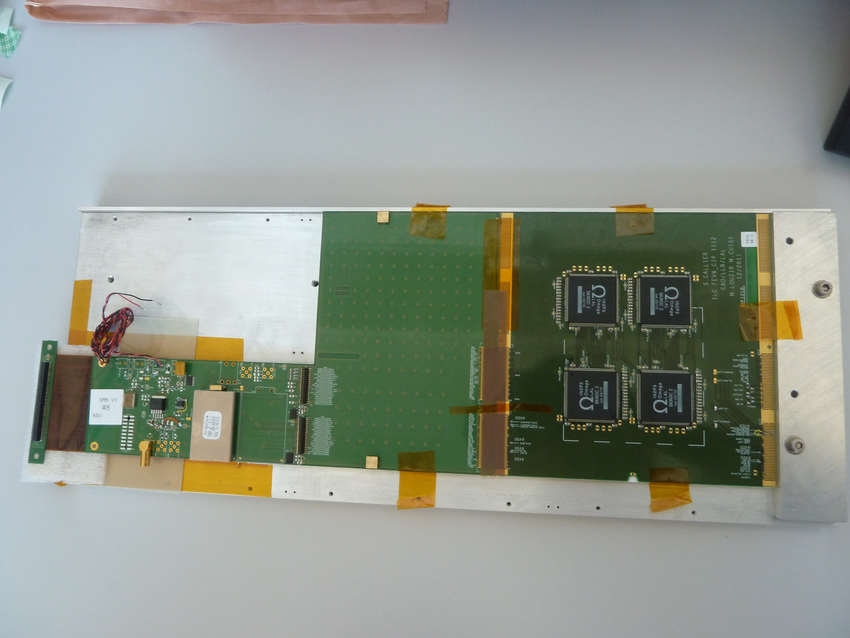
\includegraphics[width=1.\linewidth]{chap3/fig/SiW-ECAL_Techno.png}
    \caption{} \label{fig:SiWECALTechno}
  \end{subfigure}
  \caption{\subref{fig:SiWECALPhysics}) The schematics of the SiW-ECAL physics prototype. \subref{fig:SiWECALTechno}) Picture of a layer of the SiW-ECAL technological prototype.}
\end{figure}

After the validation of the calorimeter concept, a technological SiECAL prototype is being developed focusing on the integration into a full linear collider detector. To do this, modules close to the ILD design are being developed taking into account mass-production and low-power front-end electronics are integrated into the detector volume. The silicon wafers are larger and divided into 9$\times$9 cm$^2$ sensors. The PIN diode matrix is reduced to 5$\times$5 mm$^2$ pads to improve the pattern recognition of the calorimeter. New designs to the sensor are also made to minimize dead area at the sensor edge and cross-talk effects. The front-end is equipped with an ASIC, the SKIROC2 chip \cite{1748-0221-6-12-C12040}. It has 64 channels with adjustable gain charge pre-amplifier, a 12-bit ADC and digital logic. Also, it allows for auto-triggering with adjustable threshold (below 0.5 MIP) and hit time recording performed on a 12-bit TDC ramp. The SKIROC2 ASIC is designed to match the ILC beam structure (see section \ref{}) and thus allows for a power-pulsed mode where electronics are switched off between ILC bunches. This allows a very low power dissipation in the order of 25 \si{\micro\watt} per channel.

\subsection{ScECAL}
\label{subsec:ScECAL}

\section{Hadronic Calorimeters}

\subsection{AHCAL}
\label{subsec:SPIROC2B}

\subsection{SDHCAL}
\subsection{DHCAL}
